% Split in several slides and add a diagram or photo
\section{Goals}

\begin{frame}
\frametitle{Considered issues}

The ALMA project, which when fully operational will generate over 1TB of data per observation day. So, we consider the
following issues:

\begin{itemize}
	\item \textbf{Storage}, is necessary to have data center capable of storage according the data consumption needs.
\end{itemize}

\begin{center}
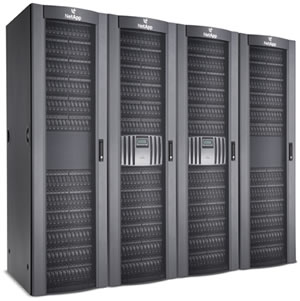
\includegraphics[height=0.3\textheight]{img/storage}
\end{center}

\end{frame}


\begin{frame}
\frametitle{Considered issues}
\begin{itemize}
	\item \textbf{Access}, in this project it has been decided that a web system is an appropriate mechanism to supply
		this requirement.
\end{itemize}

\begin{center}
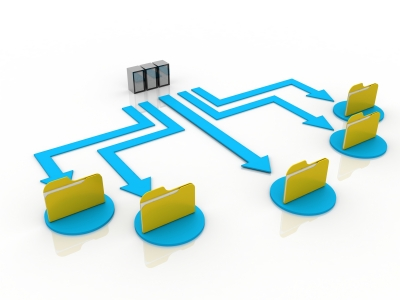
\includegraphics[height=0.3\textheight]{img/access}
\end{center}

\end{frame}


\begin{frame}
\frametitle{Considered issues}
\begin{itemize}
	\item \textbf{Processing}: Having large volumes of data, the processing to accomplish, requires more time than usual
		and computational resources. So a computational cluster, can be an useful tool to facilitate this work.
\end{itemize}

\begin{center}
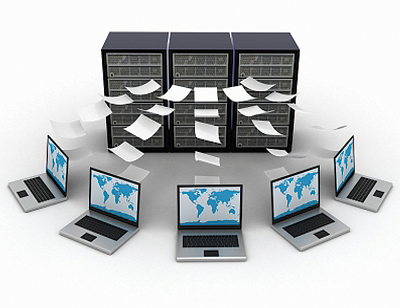
\includegraphics[height=0.3\textheight]{img/processing}
\end{center}

\end{frame}
